%%%%%%%%%%%%%%%%%%%%%%%%%%%%%%%%%%%%%%%%%
% Beamer Presentation
% LaTeX Template
% Version 1.0 (10/11/12)
%
% This template has been downloaded from:
% http://www.LaTeXTemplates.com
%
% License:
% CC BY-NC-SA 3.0 (http://creativecommons.org/licenses/by-nc-sa/3.0/)
%
%%%%%%%%%%%%%%%%%%%%%%%%%%%%%%%%%%%%%%%%%

%----------------------------------------------------------------------------------------
%	PACKAGES AND THEMES
%----------------------------------------------------------------------------------------

\documentclass[aspectratio=43,mathserif]{beamer}

\mode<presentation> {

% The Beamer class comes with a number of default slide themes
% which change the colors and layouts of slides. Below this is a list
% of all the themes, uncomment each in turn to see what they look like.

%\usetheme{default}
%\usetheme{AnnArbor}
%\usetheme{Antibes}
%\usetheme{Bergen}
%\usetheme{Berkeley}
%\usetheme{Berlin}
%\usetheme{Boadilla}
%\usetheme{CambridgeUS}
%\usetheme{Copenhagen}
%\usetheme{Darmstadt}
%\usetheme{Dresden}
%\usetheme{Frankfurt}
%\usetheme{Goettingen}
%\usetheme{Hannover}
%\usetheme{Ilmenau}
%\usetheme{JuanLesPins}
%\usetheme{Luebeck}
\usetheme{Madrid}
%\usetheme{Malmoe}
%\usetheme{Marburg}
%\usetheme{Montpellier}
%\usetheme{PaloAlto}
%\usetheme{Pittsburgh}
%\usetheme{Rochester}
%\usetheme{Singapore}
%\usetheme{Szeged}
%\usetheme{Warsaw}

% As well as themes, the Beamer class has a number of color themes
% for any slide theme. Uncomment each of these in turn to see how it
% changes the colors of your current slide theme.

%\usecolortheme{albatross}
%\usecolortheme{beaver}
%\usecolortheme{beetle}
%\usecolortheme{crane}
%\usecolortheme{dolphin}
%\usecolortheme{dove}
%\usecolortheme{fly}
%\usecolortheme{lily}
%\usecolortheme{orchid}
%\usecolortheme{rose}
%\usecolortheme{seagull}
%\usecolortheme{seahorse}
%\usecolortheme{whale}
%\usecolortheme{wolverine}

%\setbeamertemplate{footline} % To remove the footer line in all slides uncomment this line
%\setbeamertemplate{footline}[page number] % To replace the footer line in all slides with a simple slide count uncomment this line

%\setbeamertemplate{navigation symbols}{} % To remove the navigation symbols from the bottom of all slides uncomment this line
}

\usepackage{graphicx} % Allows including images
\usepackage{booktabs} % Allows the use of \toprule, \midrule and \bottomrule in tables
\usepackage{lmodern} %Lucida Modern font...
\usepackage{gensymb} %Get the bloody degree symbol...
\usepackage[style=apa]{biblatex}
\usepackage{hyperref} %Typeset URLs correctly. Grrr.
\usepackage{breakurl} % Ditto. Double Grrrr.
\bibliography{fghorow}


%----------------------------------------------------------------------------------------
%	TITLE PAGE
%----------------------------------------------------------------------------------------

\title[Gravitational Tomography]{Gravitational Tomography of the Earth; \\A Work In Progress } % The short title appears at the bottom of every slide, the full title is only on the title page

\author{Frank Horowitz} % Your name
\institute[Cornell] % Your institution as it will appear on the bottom of every slide, may be shorthand to save space
{
Cornell University\\ % Your institution for the title page
\medskip
\textit{frank.horowitz@cornell.edu} % Your email address
}
\date{April 22, 2016} % Date, can be changed to a custom date

\begin{document}

\begin{frame}
\titlepage % Print the title page as the first slide

{\footnotesize This work was performed with applied math undergrad Korin Carpenter of the University of Rochester as well as with geodetic advice from Gabriel Strykowski of the Technical University of Denmark. However, blame only me for mistakes!}
\end{frame}

\begin{frame}
\frametitle{Overview} % Table of contents slide, comment this block out to remove it
\tableofcontents % Throughout your presentation, if you choose to use \section{} and \subsection{} commands, these will automatically be printed on this slide as an overview of your presentation
\end{frame}

%----------------------------------------------------------------------------------------
%	PRESENTATION SLIDES
%----------------------------------------------------------------------------------------

%------------------------------------------------
\section{Theoretical Motivation} % Sections can be created in order to organize your presentation into discrete blocks, all sections and subsections are automatically printed in the table of contents as an overview of the talk
%------------------------------------------------

\subsection{Gravitational Potential}
\begin{frame}
\frametitle{Reminder: $1/r$ Potential}

The Newtonian gravitational \emph{potential} due to a point mass is given by
$$V(x_1) = \frac{-G \/m(x_2)}{r_{12}}$$
where $V$ is the potential evaluated at position $x_1$, $G$ is the Newtonian gravitational constant, $m$ is a mass located at position $x_2$, and $r_{12} \equiv  ||\vec{x_1} - \vec{x_2}||$ is the (Euclidean) distance from $x_1$ to $x_2$.

It's the Green's function for the Poisson's equation governing classical gravitation. (This has the form of the classical $1/r$ potential for a \emph{centrally directed force}.)

\end{frame}

\begin{frame}
\frametitle{Spatially Distributed Mass}

If the mass is spatially distributed, that potential can be re-stated as a convolution between the mass distribution and $\frac{1}{r_{12}}$: 

\[V(x_1) = -G \left(m(x_2) * \frac{1}{r_{12}}\right)\]

\end{frame}

\begin{frame}
\frametitle{EGM2008}

\begin{itemize}

\item There is a \emph{model} for the Earth's gravitation called Earth Gravitational Model 2008 (EGM2008)\footfullcite{EGM2008PavlisEtAl12}. 

\item It combines surface measurements over land, gravity estimated from sea-surface height measurements over the oceans, airborne measurements over ice sheets, and satellite measurements (e.g. GRACE, GOCE) into a uniform gravity model.

\item EGM2008 expresses a potential in spherical harmonics (SH) complete to degree and order 2159 and including some information out to order 2190.

\item For our purposes, we'll treat this model as \emph{data}.  
\end{itemize}

\end{frame}

\begin{frame}
\frametitle{EGM2008 -- Raw Potential}

\begin{figure}
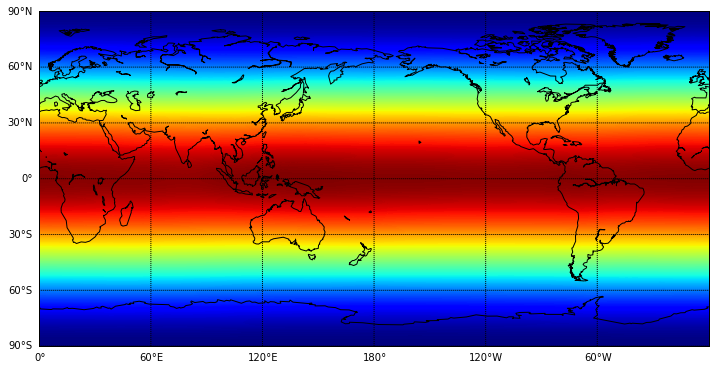
\includegraphics[width=0.9\linewidth]{EGM08Raw.png}
\end{figure}

My first surprise! They needed 2159 SH degrees and orders for \emph{that}? This shortly will lead to some considerations from physical geodesy. But first we need some SH math.

\end{frame}


\subsection{Spherical Harmonics} % A subsection can be created just before a set of slides with a common theme to further break down your presentation into chunks

\begin{frame}
\frametitle{Spherical Harmonics (Pretty Pictures)}
\begin{figure}

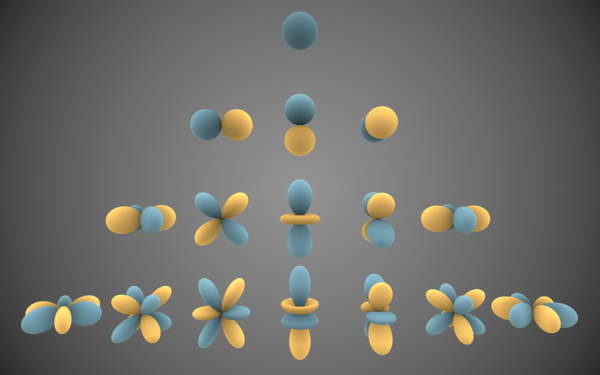
\includegraphics[width=0.4\linewidth]{Spherical_Harmonics.png}
\end{figure}

\begin{figure}
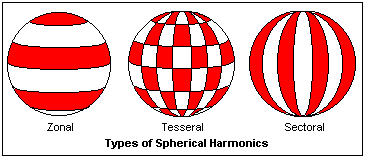
\includegraphics[width=0.4\linewidth]{harmosZonalSectoral.png}
\end{figure}
\end{frame}

\begin{frame}
\frametitle{Spherical Harmonics (Pretty Equations :-)}
Any real, square-integrable function $f$ on the sphere  may be expressed in terms of a Spherical Harmonic (SH) series:
$$ f(\theta,\phi) = \sum_{l=0}^\infty \sum_{m=-l}^{l} f_{l m} Y_{l m}(\theta,\phi)$$
where $\theta$ is the co-latitude (0\degree\/ at the North Pole, and 180\degree\/ at the South Pole), and $\phi$ is the longitude, $Y_{l m}(\theta,\phi)$ are the SH basis functions -- the first few of which were shown in the previous slide, and $f_{l m}$ are the transform coefficients.

\end{frame}

\begin{frame}
\frametitle{SH Basis Functions ($Y_{l m}$)}

The basis functions themselves are defined as follows:
$$ Y_{l m}(\theta,\phi) = \begin{cases} 
\bar{P}_{lm}(\cos \theta) \cos m \phi & \mbox{if } m \ge 0 \\
\bar{P}_{l \/|m|}(\cos \theta) \sin |m| \phi & \mbox{if } m < 0
\end{cases}$$
Here, the $\bar{P}_{lm}$ are the normalized associated Legendre functions.
\end{frame}

\begin{frame}
\frametitle{Normalized Associated Legendre functions ($\bar{P}_{l m}$)}
In turn, the normalized associated Legendre functions are defined as:
$$ \bar{P}_{lm}(\mu) = \sqrt{\frac{(2 - \delta_{m0})(2 l + 1)}{4 \pi} \frac{(l-m)!}{(l+m)!}} P_{lm}(\mu)$$
where \(\mu = \cos \theta\), \(\delta_{m0}\) is Kronecker's delta, and:
\begin{eqnarray*}
P_{lm}(\mu) &= &(1-\mu^2)^{m/2} \frac{d^m}{d\mu^m} P_l(\mu) \\
P_l(\mu) &= &\frac{1}{2^l l!} \frac{d^l}{d\mu^l} (\mu^2 -1)^l
\end{eqnarray*}
Here, \(P_l(\mu)\) are the Legendre polynomials.

Tracing back through those definitions, we'll shortly need:
\[
Y_{l0}(\theta,\phi) = \bar{P}_{l0}(\mu) = \sqrt{\frac{2l + 1}{4 \pi}} P_{l0}(\mu) = \sqrt{\frac{2l + 1}{4 \pi}}P_l(\mu)
\]

\end{frame}


\begin{frame}
\frametitle{SH Normalization Conventions}
There are a number of normalization conventions for Spherical Harmonics. 

\emph{BE CAREFUL!}

Physical geodesists use (and EGM2008 is represented in) a so-called \(4\pi\) normalization convention.

The SH convolution theory to follow is in a fully orthonormalized convention. Physicists and seismologists also occasionally throw in something called Condon-Shortley phase \((-1)^m\), which alternates signs depending on whether \(m\) is even or odd.

What I did was perform all of the geodetic processing in the geodetic convention, then convert the resulting grid to the fully orthonormalized convention (using the Condon-Shortley phase), so that I could apply the convolution theory under the convention in which it was derived. In fact, the \(P_{l0}\) expression in the last slide was already in the fully orthonomalized convention.

(This stuff will drive you mad!)


\end{frame}

\begin{frame}
\frametitle{SH Convolution}
\begin{itemize}

\item Recall from a few slides back that we will need to convolve an EGM2008 derived potential with \(1/r\) -- ideally in the SH domain. 

\item In the Fourier domain, there is the well known convolution theorem that allows \emph{fast} convolutions between two functions simply as the product of their Fourier transforms. 

\item In the SH domain, a similar theorem exists. However, while one function of the convolution pair may be general, the other function is restricted to being \emph{zonal} (i.e. a function of co-latitude only). 

\end{itemize}
\end{frame}

\begin{frame}
\frametitle{SH Convolution Theorem}
The SH convolution expression is theorem 1 of Driscol and Healy\footfullcite{DriscollHealy94}. Both of the functions \(f\) and \(h\) must be square-integrable on the sphere, and \(h\) must be zonal.
\begin{theorem}[Spherical Harmonic Convolution]
\( \widehat{(f*h)}_{lm} = 2\pi \sqrt{\frac{4 \pi}{2l + 1}} \hat{f}_{lm} \hat{h}_{l0} \) 
\end{theorem}
\end{frame}

\begin{frame}
\frametitle{Geometry of \(r_{12}\)}
Because we will be convolving, we are free to  use the North Pole as the reference point on the Earth's surface where we are evaluating the potential \(V\). Fortunately, by rotational symmetry about the Earth's rotation axis, \(r_{12}\) yields a zonal function and hence -- once SH transformed -- we can insert the result into the SH convolution theorem.
\begin{figure}
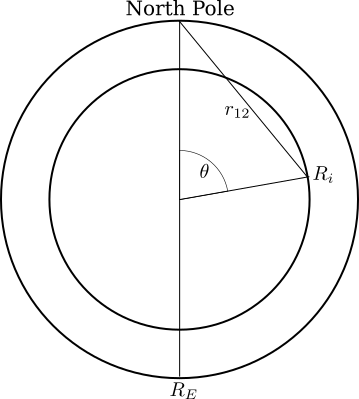
\includegraphics[width=0.35\linewidth]{EarthGeometry.png}
\end{figure}
\end{frame}

\begin{frame}
\frametitle{SH Transform of \(1/r\) (I)}
Here, we adapt the development in chapter 12 of Arfken and Weber\footfullcite{ArfkenWeber95} to our notation from the previous slides. First, we use the law of cosines to obtain:
\[\frac{1}{r_{12}} = (R^2_E +R^2_i - 2 R_E R_i \cos \theta)^{-1/2}
\]
\end{frame}

\begin{frame}
\frametitle{SH Transform of \(1/r\) (II)}

Next, after expanding the radical in a binomial series, re-arranging in powers of \(R_i/R_E\), and defining both \(\mu = \cos \theta\) and \(t = R_i / R_E\) we ultimately find:
\[g(\mu,t) = (1 - 2 \mu t + t^2)^{-1/2} = \sum_{l=0}^{\infty} P_l(\mu) t^l
\]
Here, the \(P_l(\mu)\) are Legendre polynomials as before. The function \(g(\mu,t)\) (i.e. \((1/R_E) (1/r_{12})\) ) is actually the so-called ``generating function'' of the Legendre polynomials! 

Viewed another way, that means that the  \(t^l = (R_i/R_E)^l\) are \emph{an analytic expression for the Legendre polynomial expansion of} \(1/r_{12}\) (Arfken and Weber\footfullcite{ArfkenWeber95}, p. 710). 
\end{frame}

\begin{frame}
\frametitle{SH Expansion of \(1/r\) (III)}
Pulling that all together with our expression for \(Y_{l0}\) from a few slides back, this means that the \emph{analytic expression} for the SH expansion of \(1/r_{12}\) is:
\[
\frac{1}{R_E r_{12}} = \sum_{l=0}^{\infty} \sqrt{\frac{4 \pi}{2l + 1}} (R_i/R_E)^l Y_{l0}(\theta,\phi)
\]
As a reminder, this is a zonal function ready to be used in the SH convolution theorem.
\end{frame}

\begin{frame}
\frametitle{SH Expansion of \(1/r\) (IV)}
Just for confidence in this result, here is a plot of \(1/r_{12}\) from the SH expansion of the previous result for an inner sphere at a depth of 150 km.

\begin{figure}
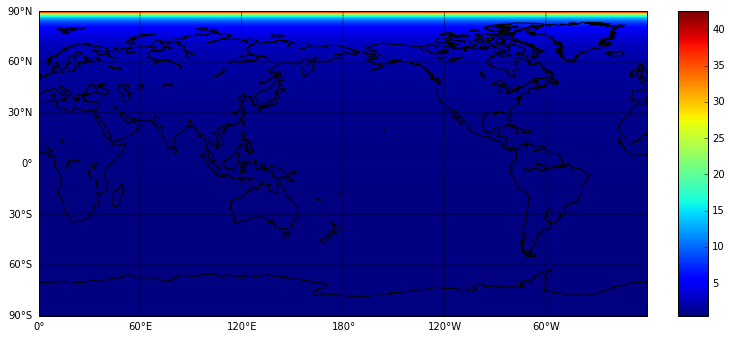
\includegraphics[width=0.9\linewidth]{OneOnR150km.png}
\end{figure}


\end{frame}

\begin{frame}
\frametitle{SH Software}
\begin{itemize}
\item I am using the open-source software package SHTools\footfullcite{SHTools}. 

\item It is quite flexible, supporting the major normalization conventions. In particular, it uses stable algorithms for evaluating high degree Legendre polynomials, and has a routine that estimates the geoid from EGM2008 coefficients.

\item It has its quirks, but it does appear to work. Most of the non-trivial problems I've had with it have been errors on my part, not the software.

\item I was drawn to it because it has a Python binding that lets me work with it from NumPy.
\end{itemize}
\end{frame}

\subsection{Geodetic Considerations}
\begin{frame}
\frametitle{EGM2008 and Physical Geodesy}
Recall this plot of the contents of EGM2008:
\begin{figure}
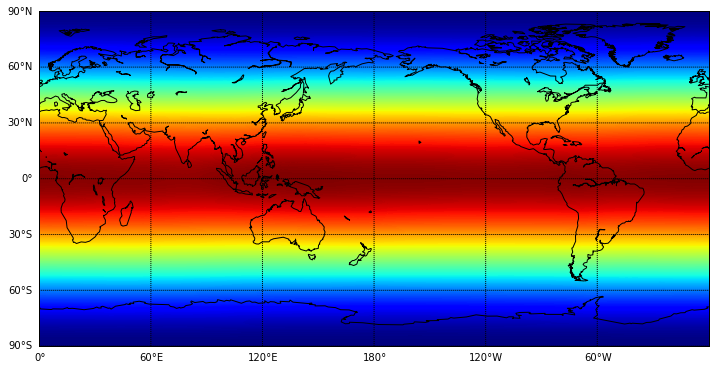
\includegraphics[width=0.9\linewidth]{EGM08Raw.png}
\end{figure}
There are \emph{many} different potentials defined in Physical Geodesy. The one expressed by EGM2008 contains at least the centripetal accelerations of the rotating planet.
\end{frame}

\begin{frame}
\frametitle{A Geoid From EGM2008}
\begin{itemize}
\item Due to the geoid's centrality in the conceptual work of Physical Geodesy, perhaps the best tested code in SHTools is the routine that evaluates the geoid from EGM2008.  Calculation of the geoid does the job of getting rid of the rotational accelerations embedded within EGM2008.

\item In addition to the SH coefficients, that geoid routine needs a reference ellipsoid. We use the GRS80 model -- an immediate ancestor of the WGS84 reference system and geodetic datum familiar from the GPS system.

\item Recall that a geoidal height is defined as the height of an equipotential surface above the reference ellipsoid. We'll denote this geoidal height (also known as the geoidal undulation) by \(N\).
\end{itemize}

\end{frame}

\begin{frame}
\frametitle{EGM2008 from Physical Geodesy}
Here is the geoidal height \(N\) calculated from EGM2008:
\begin{figure}
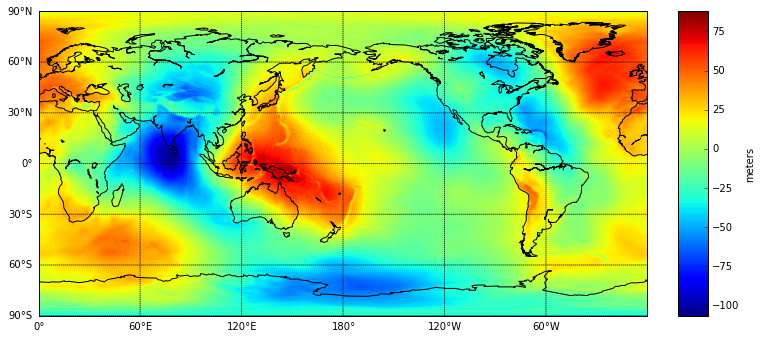
\includegraphics[width=0.9\linewidth]{geoid.png}
\end{figure}

\end{frame}

\begin{frame}
\frametitle{The Disturbing Potential \(T\) (I)}

For the purposes of solid Earth geophysics, the geodetic potential of most interest is \(T\) the (so-called) Disturbing (or Anomalous) Potential. By definition, \(T\) contains only the information from anomalous mass distributions. 

From Heiskanen and Mortiz\footfullcite{HeiskanenMoritz} (equation 2-143), \(T\) is related to \(N\)  via the so-called normal gravity \(\gamma\) -- which is the gravity computed on the reference ellipsoid due only to its shape, total mass, and rotation. The relation is:
\[ T = \gamma N
\]

This is a famous linear approximation known in physical geodesy as \emph{the Bruns formula}.


\end{frame}

\begin{frame}
\frametitle{The Normal Gravity (\(\gamma\)) for GRS80}

SHTools also has a routine to evaluate the normal gravity (\(\gamma\)) for a specified ellipsoid. Here is the result for GRS80:

\begin{figure}
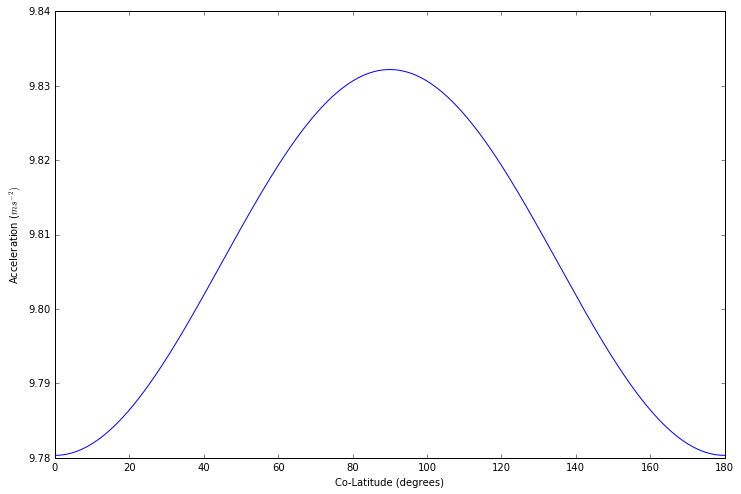
\includegraphics[width=0.8\linewidth]{NormalGravity.png}
\end{figure}

\end{frame}

\begin{frame}
\frametitle{The Disturbing Potential \(T\) (II)}

\(T\) has dimensions of energy/unit mass. Here is the result:

\begin{figure}
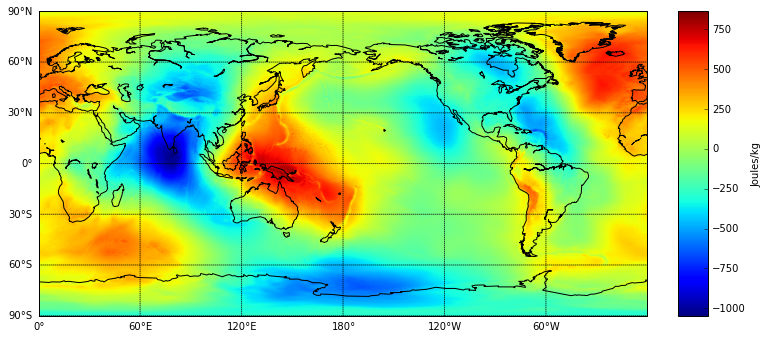
\includegraphics[width=0.9\linewidth]{TImage.png}
\end{figure}

This looks very similar to the geoid because \(\gamma\) is close enough to a constant as to be barely distinguishable in the normalized color scale.

\end{frame}

\begin{frame}
\frametitle{From Geodesy to Tomography}

That's the end of our geodetic manipulations. At this point in the processing chain, we stop using the geodetic \(4 \pi\) SH normalization convention and switch to the fully orthonomalized SH convention to make sure that we are not inadvertently violating something crucial in applying the convolution theorem.

We do this by taking the \(T\) grid, and SH transforming it using the orthonomalized (with Condon-Shortly phase) conventions in SHTools.

For a sanity check, after round-tripping \(T\) into it's orthonormalized SH representation and back out, the relative error ((\(T_{4\pi} - T_{orthonorm})/T_{4\pi}\)) between the two grids has worst case extrema between  \(-4.7 \times 10^{-6} \)  and  \(4.3 \times 10^{-6} \).  There's a lot of numerical work going on between \(T_{4\pi}\) and \(T_{orthonorm}\). That's close enough to accumulated roundoff for our purposes. 

\end{frame}

\subsection{Tomography}

\begin{frame}
\frametitle{Filtered Backprojection}
A major approach to tomographic imaging algorithms involves reconstruction by Filtered Backprojection (FBP). The key backprojection idea\footnote{The image is from \burl{http://www.owlnet.rice.edu/~elec539/Projects97/cult/node2.html} retrieved on 21 April 2016.} is very simple (even if the math gets a bit intricate).

\begin{figure}
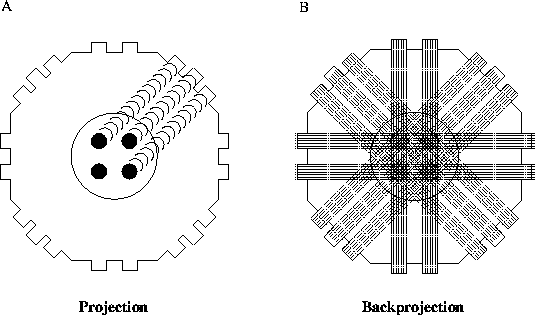
\includegraphics[width=0.45\linewidth]{BackProjection.png}
\end{figure}
The goal of the \emph{Filtering} part is to remove those stripey/blurry artifacts from backprojection.

\end{frame}

\begin{frame}
\frametitle{The History of the Idea}
\begin{itemize}
\item The basic math goes back to Radon (1917)\footfullcite{Radon1917Translation86}. 

\item In addition to the backprojection shown in the previous slide, Radon derived an optimal filter that `de-blurs' the result.

\item It's probably fair to say that this idea lies at the conceptual heart of all modern tomographic medical imaging technologies (even if their implementation varies).

\item It turns out (in abstract form at least; see Dave Hysell's class poster!) to also underly several algorithms from geophysics. However, this current work is probably the application with the best geometrical coverage in solid Earth geophysics.
\end{itemize}
\end{frame}

\begin{frame}
\frametitle{The \emph{Discrete} Radon Transform}

\begin{itemize}

\item Beylkin (1987)\footfullcite{Beylkin87} took the Radon transform and generalized the theory, both into a discrete formulation and into very general manifolds on which the integration can be performed.  He also derives an optimal filter for FBP.

\item In particular, integrating over a sphere is allowable.

\item Because of the fast SH convolution, this is an attractive computational route to working through our problem, and it is the approach we use here.

\end{itemize}

\end{frame}

\begin{frame}
\frametitle{`Operators' for Our Problem}

\begin{itemize}

\item In our discrete problem `operators' are conceptually matrices convolutionally mapping input vectors to output vectors. Conceptually the vectors, in turn, contain \(T\) on the surface (\(R_E\)) and some mass distribution (\(m_i\)) that we are attempting to image on the inner sphere (\(R_i\)).

\item The forward operator \(A_i\) maps from \(m_i\) to \(T\). 

\item The back-projection operator \(A_i^*\) maps from \(T\) to \(m_i\).

\item Because the operators are convolutional in nature, they can be expressed via the SH convolution theorem we described earlier.

\item This concept of a \emph{single} internal sphere containing \emph{all} of the mass density variation is known as a Bjerhammar sphere in physical geodesy. In flat-Earth potential fields, an analog would be an equivalent layer of mass density at some depth.


\end{itemize}
\end{frame}

\begin{frame}
\frametitle{FBP in SH (I)}
Beylkin (1987) shows that the relevant FBP inversion algorithm for discrete Radon transforms can be expressed via either one of two operator identities. In our notation the first one becomes:
\[(A_i^* A_i)^{-1}  A_i^* A_i = I\]
where \(I\) is the identity.
Right multiplying both sides by \(m_i\) and substituting \(A_i m_i = T\) we find:
\[(A_i^* A_i)^{-1} A_i^* T= m_i\]
This is the `backproject then filter' algorithm. The backprojection operator is \(A_i^*\) and the filter operator is \((A_i^* A_i)^{-1}\).
\end{frame}

\begin{frame}
\frametitle{FBP in SH (II)}
\begin{itemize}
\item Now, because we're in the SH domain, our \(\widehat{1/r_{12}}\) operator is already \emph{real and diagonal} and hence self-adjoint.

\item Hence, \(\widehat{A_i^*} = \widehat{A_i}\).  Also, because our SH transform coefficients are real everything actually commutes.

\item This  shows that the FBP  operator from the previous slide  (\((A_i^* A_i)^{-1} A_i^*\)) reduces to a deconvolution in the SH domain for this problem. (Danger Will Robinson!)


\item This means that Beylkin's second identity (\(A_i^* (A_i^* A_i)^{-1}   A_i = I \) -- the `filter then backproject' algorithm) essentially reduces to the same thing in the SH domain, and we get nothing new via deriving algorithms from it.


\end{itemize}

\end{frame}

\section{Results}
\begin{frame}
\frametitle{The Operator \(A_{10}^*\)}

Plotted here in blue is the amplitude of the EGM2008 order 0 coefficients for all degrees -- essentially the zonal component -- to give some idea of the order of magnitude of the data. Plotted in green is the amplitude of the 10 km backprojection operator coefficients.

\begin{figure}
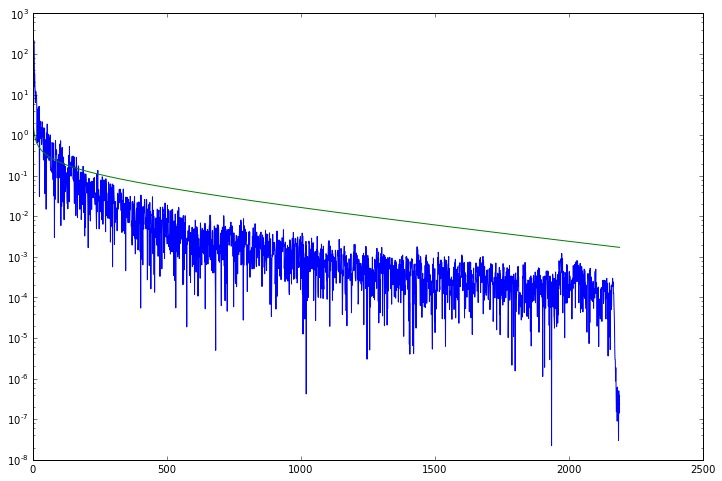
\includegraphics[width=0.7\linewidth]{1_r_10.png}
\end{figure}
\end{frame}

\begin{frame}
\frametitle{The Backprojected Data at 10 km}

\begin{figure}
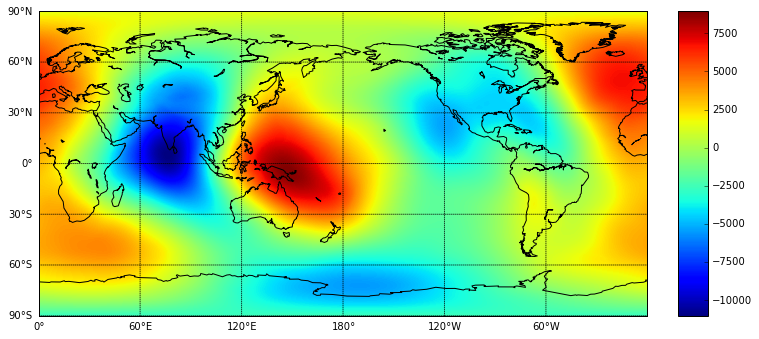
\includegraphics[width=0.9\linewidth]{BP10.png}
\end{figure}

Not much to say here other than it's pretty smooth (blurry).
\end{frame}
\begin{frame}

\frametitle{The Filtered Backprojected Image at 10 km}

\begin{figure}
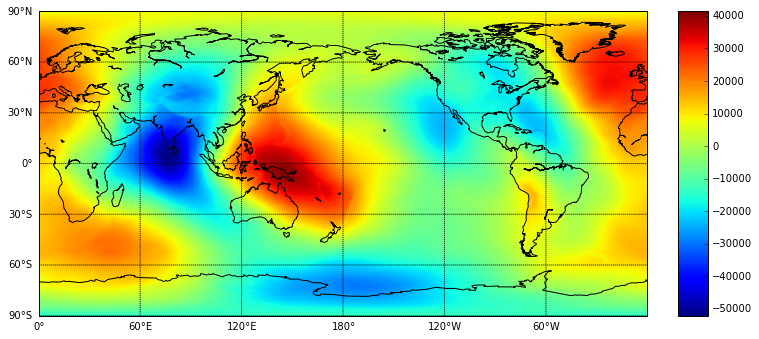
\includegraphics[width=0.9\linewidth]{FBP10.png}
\end{figure}

It's a bit sharper in some regions, exactly as you would expect from the filtering in the FBP algorithm.
\end{frame}

\begin{frame}
\frametitle{The Operator \(A_{20}^*\)}

As before, blue is EGM2008, and green is the 20 km backprojection operator. Note that the amplitudes at high degrees are nearly equal.

\begin{figure}
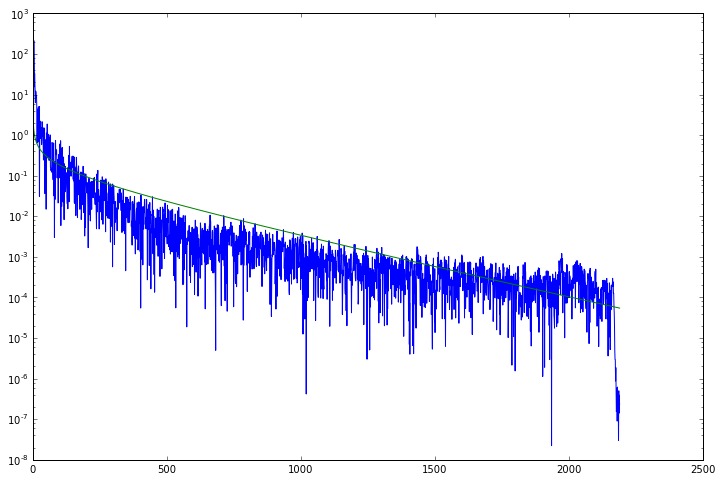
\includegraphics[width=0.65\linewidth]{1_r_20.png}
\end{figure}
\end{frame}

\begin{frame}

\frametitle{The Filtered Backprojected Image at 20 km}

\begin{figure}
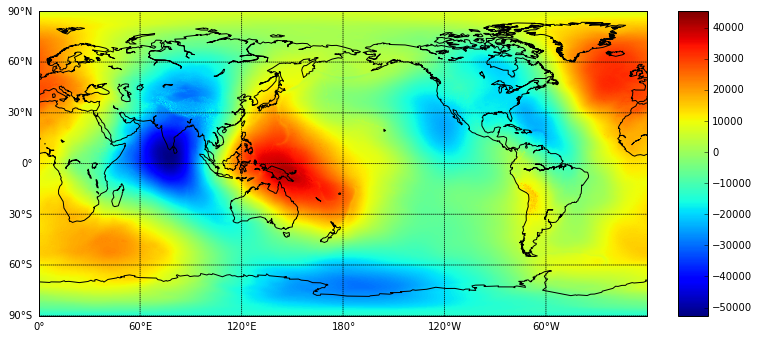
\includegraphics[width=0.9\linewidth]{FBP20.png}
\end{figure}

It's yet again sharper in some regions.
\end{frame}

\begin{frame}
\frametitle{The Operator \(A_{30}^*\)}

As before, blue is EGM2008, and green is the 20 km backprojection operator. Note that the operator amplitudes at high degrees are now significantly smaller than the EGM2008 data. That means when squared and inverted in the filter operator, they start to significantly amplify the high degree features.

\begin{figure}
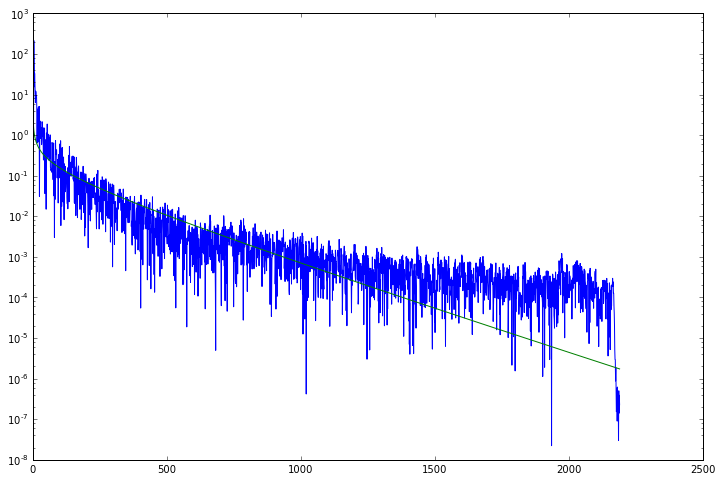
\includegraphics[width=0.65\linewidth]{1_r_30.png}
\end{figure}
\end{frame}

\begin{frame}

\frametitle{The Filtered Backprojected Image at 30 km}

\begin{figure}
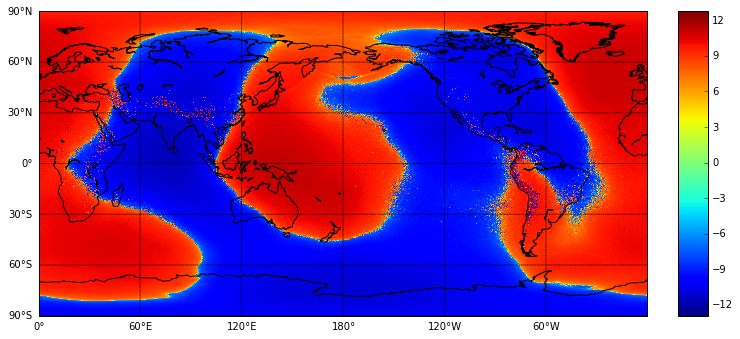
\includegraphics[width=0.9\linewidth]{FBP30.png}
\end{figure}

The image has now gone unstable! (Already! At only 30 km depth!) I had to log-stretch the scale (technically, \(sinh^{-1}\) to allow for negative numbers) to even display this. It gets worse with increasing depth.
\end{frame}

\begin{frame}
\frametitle{Snoopy Said it Best\footnote{The image is from \burl{http://www.cafepress.com/+flying_ace_rats_shower_curtain,1272017624} retrieved on 21 April 2016.}}

\begin{figure}

\includegraphics[width=0.5\linewidth]{flying_ace_rats_shower_curtain.jpg}
\end{figure}

\end{frame}

\begin{frame}
\frametitle{Drawbacks of our Approach}

\begin{itemize}

\item \emph{The imaging operator turned out to be unstable!}
\item By concentrating all of the mass on to a single inner spherical shell, we are neglecting the fact that this is unphysical. (The idea was to see if anything interpretable resulted anyway.)

\item That concentration leads to Gibb's phenomena-like ringing.

\item Those are the primary reasons why I'm calling this ``a work in progress''.

\end{itemize}
\end{frame}


%------------------------------------------------

\begin{frame}
\Huge{\centerline{The End}}
\end{frame}

%----------------------------------------------------------------------------------------

\end{document}